\documentclass[a4paper]{book}

% packages % 
\usepackage[utf8]{inputenc} 
\usepackage{fvextra}
\usepackage{csquotes}
\usepackage[french, italian, spanish, english]{babel}
\usepackage[T1]{fontenc}   
\usepackage{color}  
\usepackage{amsmath, dsfont, amssymb, amsthm, stmaryrd}
\usepackage[style=alphabetic]{biblatex}
\usepackage{enumitem}
\usepackage[hidelinks]{hyperref}

% graphics %
\usepackage{graphicx}
\graphicspath{ {./images/} }

% environments %
\newtheorem{theorem}{Theorem}[section]
\newtheorem{corollary}{Corollary}[theorem]
\newtheorem{lemma}[theorem]{Lemma}

\theoremstyle{definition}
\newtheorem{definition}{Definition}[section]

\theoremstyle{remark}
\newtheorem*{remark}{Remark}
\newtheorem*{example}{Example}



% bibliography %
\bibliography{bibliography} 

\begin{document}

% title %
\title{General Relativity}
\author{Buisine Léo\\Ecole Normale Superieure of Paris}
\maketitle

\tableofcontents

\chapter{Introduction}
Danièle Steer: daniel.steer@phys.ens.fr \newline
work on theories of gravity, gravitational waves, primordial cosmology \par \medskip 

We should do the TD before the TD. \par \medskip 

This will be a course more physical than mathematical. No differential geometry or Cartan geometry. The TD will be more formal. The objective is to understand current experiments and current measures. As such, we will mostly stay outside of black holes horizons. We will also use cevtors in coordinate basis. We should remember that physics is independant of the choice of coordinates. The objective is to be able to do accurate computations.\par \bigskip 

Aims:
\begin{enumerate}
    \item Handle GR and its tools
    \item Be able to do accurate calculations 
    \item Have a feeling for different works in GR today
\end{enumerate} \bigskip 

The current GR fails at cosmological scale. It doesn't explain the Hubble constant, Dark energy nor Dark matter. Many theories try to modify GR, but many of these modified gravities are constantly ruled out by new experiments and new data. For exemple, a whole lot of theories were ruled out in 2017 by an experiment showing that 
\begin{equation}
    \left|\frac{c_{GW}-c}{c}\right| < 10^{-15}
\end{equation}\par \medskip 

The Newtonian gravity potential on the surface of a body of mass $M$ and radius $R$ is given by 
\begin{equation}
    \Phi_N = \frac{GM}{R}
\end{equation}
The Newtonian gravity is valid in the limit $\Phi_N << 1$. 
\begin{enumerate}
    \item On earth, we have $\Phi_N \sim 10^-9$
    \item On the sun, we have $\Phi_N \sim 10^-6$
    \item On a neutron star, we have $\Phi_N \sim 10^-1$
    \item In a black hole, there is no upper limit
\end{enumerate}\bigskip \par \medskip 

Semi classical gravity is doing QFT in curved spacetime. The idea is to start with a classical solution of Einstein's equation. Then we quantise the field in this metric. Then we can loop, compute the change in the metric due to the field, then re quantise the field, etc... The result of this computation gives the famous Hawking temperature of black holes 
\begin{equation}
    T_H = \frac{\bar{h}c^3}{8\pi GMk_B}
\end{equation}
For a BH of mass of the sun $M_\Theta$, $T_H \sim 10^{-8}$K. This causes the decay of black holes such as primordial black holes.\par \medskip 

GR is a very unique theory. Therem of lovelock (1972): Einstein's equations are the unique 2nd order local equation of motion for a metric $g_{\mu\nu}$ derivable from an action in 4D. \par 

So if we want to go beyond GR, we can either work in more than 4D, add extra fields (ex scalar-tensor theories of gravity), we can try higher order equations of motion, or we can remove the locality. 
\chapter{Overview}
\section{Special Relativity}

For our Minkowski metric, we will take the signature $(-, +, +, +)$. SR describes all forces apart from gravity, and they live on a fixed Minkowski spacetime. \par \medskip 

In SR, there is a class of globally defined non-accelerating inertial observers, with associated pseudo-cartesian coords 
\begin{equation}
    x^\mu = (ct, x, y, z) \qquad \eta_{\mu\nu} = \text{diag}(-1, 1, 1, 1)
\end{equation}
IN GR, gravitational force is a manifestation of curvature $\eta_{\mu\nu} \rightarrow g_{\mu\nu}(x)$, given by Einstein's equation 
\begin{equation}
    G_{\mu\nu} = \frac{8\pi G}{c^4}T_{\mu\nu}
\end{equation}
We have $\frac{8\pi G}{c^4} \sim 10^{43}$. $G_{\mu\nu}$ is intrisicly related to the curvature of spacetime, by the RIemann tensor for exemple. It has dimension inverse length square? $T_{\mu\nu}$ is the energy-momentum tensor. \par \medskip 

We have 2nd order non-linear PDE for $g_{\mu\nu}(x)$. To find the solutions, we can impose symmetries 

\begin{enumerate}
    \item Cylinder symmetry: string-like BH
    \item Time independant spherical symmetry: Schwarchild BH 
    \item Planar symmetry: Domorin-Wall cosmological solution in 5D, it is a modified gravity theory
\end{enumerate}

Another idea is to do perturbative physics, and to find perturbative solutions. 
\begin{equation}
    g_{\mu\nu}(x) = \bar{g}_{\mu\nu}(x) + \delta g_{\mu\nu}(x)
\end{equation}
$\bar{g}_{\mu\nu}$ is a known solution, but can be a lot of things. Either Minkowski spacetime, either Schwarchild blackhole, either FRWL, ... \par \medskip 

Another possibility to solve the equations is when $\Phi_N << 1$, where we have 
\begin{equation}
    \triangledown ^2 \Phi = 4\pi G\rho  
\end{equation}
with $\rho$ the mass density. \par \medskip 

Geodesic equation for test masses, subject only to gravity. 
\begin{equation}
    \frac{\text{d}^2x^\mu}{\text{d}\lambda^2} + \Gamma^\mu_{\alpha\beta} \frac{\text{d}x^\alpha}{\text{d}\lambda} \frac{\text{d} x^\beta}{\text{d}\lambda} = 0
\end{equation}
equation for $x^\mu(\lambda)$, the world line of the test mass $(m>0)$, where $\lambda$ is the time perceived by the body following the geodesic, an (often, but not always: see 1st TD) affine parameter of the proper time. \par \medskip 

The Christoffel symbol is given by 
\begin{equation}
    \Gamma^\mu_{\alpha\beta} = \frac{1}{2}g^{\mu\nu} (\partial_\alpha g_{\nu\beta} + \partial_\beta g_{\nu\alpha} - \partial_\nu g_{\alpha\beta})
\end{equation}\par \medskip 

In the limit $\Phi_N << 1$, it reduces to $\vec{a} = - \vec{\triangledown} \Phi_N$. This is independant of the composition of the particle (universal equation). It is a consequence of $m_i = m_g$. THe current experiments say that 
\begin{equation*}
    \left|\frac{m_i - m_g}{m_g}\right| \sim 10^{-15}
\end{equation*}
Weak equivalence principle: $m_i = m_g$. \par \medskip 

In GR, a consequence of the WEP is that locally, gravity and acceleration are indistinguishable. Locally, the effect of gravity can be removed by going to a locally freely falling frame (LFFF).\par 
Einstein's EP: in the LFFF, the laws of physics are those of SR. Locally, $g_{\mu\nu} \sim \eta_{\mu\nu}$. 

\section{Rindler's space}

A few work on SR and Rindler Space
\begin{itemize}
    \item $x^\mu = (t, x, y, z)$ associate to globally defined non accelerating inertial observer 
    \item $\eta_{\mu\nu} = \text{diag}(-, +, +, +)$
    \item different inertial frames related by Lorentz transformations $x'^\mu = \Lambda ^\mu_\nu x^\nu$
    \item Free massive particles satisfy $\frac{\text{d}^2x^\mu}{\text{d}\tau^2} = 0$ where $\tau$ is the proper time, $ds^2 = -d\tau^2$
\end{itemize}

Now let's work in general curvilinear coords 
\begin{equation}
    x^\mu \rightarrow y^\mu(x^\alpha) \text{(assumed invertible)}
\end{equation}
\begin{example}
    spherical polar coords $y^\alpha = (t, r, \theta, \phi)$
\end{example}
\begin{example}
    Rindler: $y^\alpha = (\eta, \rho, y, z)$
\end{example}
\underline{Metric}: 
\begin{equation}
    ds^2 = \eta_{\mu\nu} \text{d}x^\mu \text{d}x^\nu = \eta _{\mu\nu} \frac{\partial x^\mu}{\partial y ^\alpha} \frac{\partial x^\nu}{\partial y ^\beta} \text{d} y^\alpha \text{d}y ^\beta
\end{equation}
with 
\begin{equation}
    \eta _{\mu\nu} \frac{\partial x^\mu}{\partial y ^\alpha} \frac{\partial x^\nu}{\partial y ^\beta}  = g_{\alpha\beta}(y)
\end{equation}
The inverse is 
\begin{equation}
    g^{\alpha\beta} = \eta ^{\mu\nu} \frac{\partial y ^\alpha}{\partial x^\mu} \frac{\partial y ^\beta}{\partial x^\nu} 
\end{equation}
Check 
\begin{equation}
    g^{\alpha\beta}g_{\beta\gamma} = \delta^\alpha_\gamma
\end{equation}

In the new coord system, $\frac{\text{d}^2x^\mu}{\text{d}\tau^2} = 0$. So 
\begin{equation}
    \frac{\text{d}^2y^\mu}{\text{d} \tau^2} + \tilde{\Gamma}^\mu_{\alpha\beta}\frac{\text{d}y^\alpha}{\text{d}\tau}\frac{\text{d}y^\beta}{\text{d}\tau} = 0
\end{equation}
where 
\begin{equation}
    \tilde{\Gamma}^\mu_{\alpha\beta} = \frac{\partial y^\mu}{\partial x^\omega} \frac{\partial^2 x^\omega}{\partial y^\alpha\partial y^\beta } = \frac{1}{2}g^{\mu\epsilon}(\partial_\alpha g_{\epsilon\beta} + \partial_\beta g_{\epsilon\alpha} - \partial_\epsilon g_{\alpha\beta})
\end{equation}
Geodesic equation, but note that we are in flat spacetime!\par \medskip 

Now consider a particular class of non-inertial observers, namely one with constant eternal proper acceleration along $x$ axis $1/r_0$ with $r_0 > 0$. (this is very unphysical). 
\begin{figure}
    \centering
    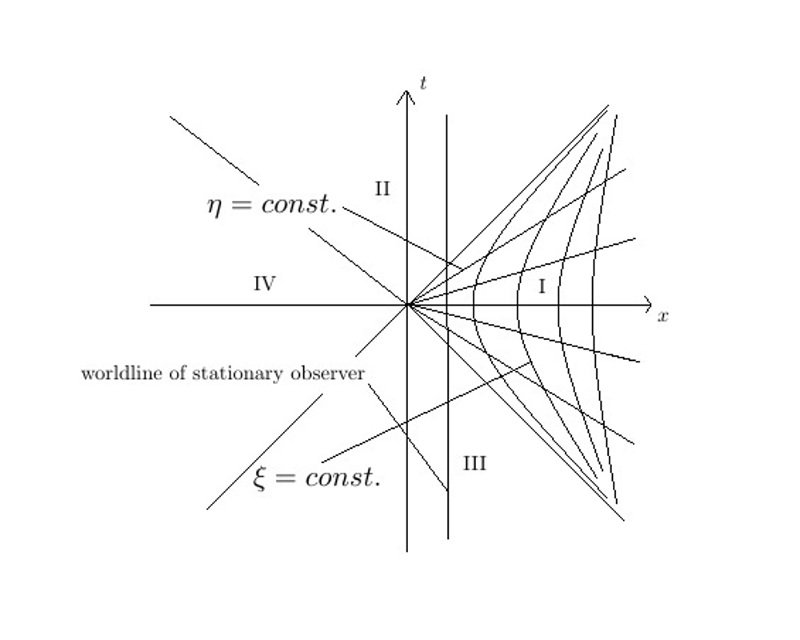
\includegraphics[width=0.7\textwidth]{rindler_coords}
    \caption{Rindler's observers}
\end{figure}
\begin{equation}
    A^\mu A_\mu = \text{const} = 1/r_0^2
\end{equation}
\begin{equation}
    A^\mu = \frac{\text{d} u^\mu}{\text{d}\tau}, \qquad u^\mu = \frac{\text{d}x^\mu}{\text{d}\tau} = (\gamma, \gamma v, 0, 0)
\end{equation}
where 
\begin{equation}
    \gamma = \frac{1}{\sqrt{1-v^2}} \quad v = \frac{\text{d}x}{\text{d}t} \quad a = \frac{\text{d}v}{\text{d}t}
\end{equation}

We can send these Rindler observers in space, resulting in the trajectories 
\begin{equation}
    \begin{aligned}
        &t = r_0 ~ \text{sinh}(\eta)\\
        &x = r_0 ~ \text{cosh}(\eta)
    \end{aligned}
\end{equation}
with $\eta = \tau/r_0$

The Rindler space is the space occupied by the trajectory of the Rindler observers, corresponding to the right wedge of the Minkowski spacetime. \par \medskip 
This allows us to parametrize the right wedge of the Minkowski spacetime, as 
\begin{equation}
   \begin{aligned}
    &t = \rho ~ \text{sinh}(\eta) \\
    &x = \rho ~ \text{cosh}(\eta)
   \end{aligned}
\end{equation}
These give the Kindler coordinates $(\rho, \eta, y, z)$ with $\rho > 0$ and $-\infty < \eta < + \infty$. In these coords, 
\begin{equation}
    \text{d}s^2 = -\rho^2 \text{d}\eta^2 + \text{d}\rho ^2 + \text{d}y^2 + \text{d}z^2
\end{equation}
Sometimes, we write $\rho = e^\chi$ in which case 
\begin{equation}
    \text{d}s^2 = e^{2\chi}\left(-\text{d}\eta^2 + \text{d}\chi^2 \right) + \text{d}y^2 + \text{d}z^2
\end{equation}\bigskip 

Now, let's look at the Schwarchild metric. For $r > r_s$
\begin{equation}
    \text{d}s^2 = -\left(1-\frac{r_s}{r}\right)\text{d}t^2 + \frac{1}{(1-\frac{r_s}{r})}\text{d}r^2 + r^2\text{d}\Omega^2
\end{equation}
where $r_s = 2GM$ and 
\begin{equation}
    \text{d}\Omega^2 = \text{d}\theta^2 + \sin^2(\theta) \text{d}\phi^2
\end{equation}
We want to consider the Schwarchild metric very near the BH horizon. We expand at first order $r = r_s + \varepsilon$
\begin{equation}
    \text{d}s^2 = -\frac{\varepsilon}{r_s}\text{d}t^2 + \frac{r_s}{\varepsilon}\text{d}\varepsilon^2 + r_s^2\text{d}\Omega^2
\end{equation}
Let 
\begin{equation}
    \begin{aligned}
        &\rho = 2\sqrt{r_s\varepsilon}\\
        & \text{d}\rho = \sqrt{\frac{r_s}{\varepsilon}}\text{d}\varepsilon
    \end{aligned}
\end{equation}
We have 
\begin{equation}
    \text{d}s^2 = -\frac{\rho^2}{4r_s^2}\text{d}t^2 + \text{d}\rho^2 + r_s^2\text{d}\Omega^2
\end{equation}
So with 
\begin{equation}
    \eta = \frac{t}{2r_s}
\end{equation}
We get 
\begin{equation}
    \text{d}s^2 = -\rho^2\text{d}\eta^2 + \text{d}\rho^2 + r_s^2\text{d}\Omega^2
\end{equation}
Which is, for the particular part, exactly the Rindler metric. So the Rindler space modelizes at first order the exterior near horizon of a black hole.


\end{document}